\section*{سوال ۱}

طراحی و پیاده سازی یک سامانه Air Conditioning با دو Super-State با زبان برنامه نویسی دلخواه و ارائه یک گزارش از روند پیاده‌سازی. توجه کنید که برای فعال کردن heater بایستی سه حالت کاری و برای فعال کردن cooler سه حالت کاری در نظر بگیرید.

\section*{جواب سوال ۱}

\begin{figure}[h]
	\centering
	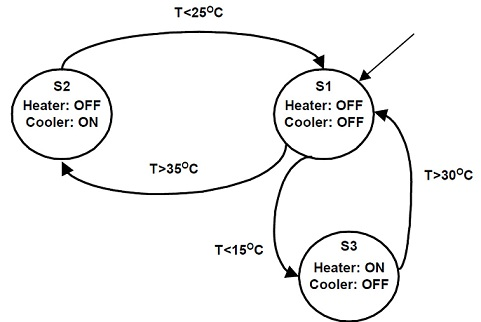
\includegraphics{6.jpg}
	\label{fig:label4}
\end{figure}

\begin{figure}[h]
	\centering
	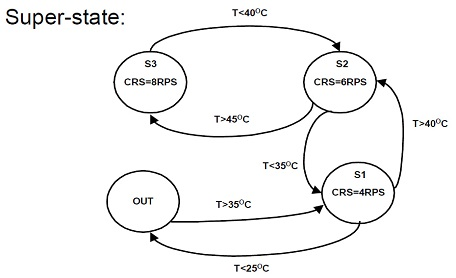
\includegraphics{7.jpg}

	\label{fig:label4}
\end{figure}

\section*{توضیح منطق انکوباتور}

\begin{enumerate}
	\item \textbf{وضعیت‌ها (States)}:
	\begin{itemize}
		\item \texttt{S1}: وضعیت اولیه
		\item \texttt{S2}: وضعیت دومی
		\item \texttt{S3}: وضعیت سومی
	\end{itemize}
	
	\item \textbf{منطق وضعیت‌ها}:
	\begin{itemize}
		\item اگر وضعیت فعلی (\texttt{PS}) برابر با \texttt{S1} باشد:
		\begin{itemize}
			\item اگر دما (\texttt{T}) بیشتر از 35 باشد، وضعیت بعدی (\texttt{NS}) به \texttt{S2} تغییر می‌کند و وضعیت زیرین \texttt{S2} به \texttt{S1} تنظیم می‌شود.
			\item اگر دما کمتر از 15 باشد، وضعیت بعدی به \texttt{S3} تغییر می‌کند و وضعیت زیرین \texttt{S3} به \texttt{S1} تنظیم می‌شود.
			\item در غیر این صورت، وضعیت بعدی همچنان \texttt{S1} است.
		\end{itemize}
		\item اگر وضعیت فعلی برابر با \texttt{S2} باشد:
		\begin{itemize}
			\item وضعیت زیرین بر اساس وضعیت فعلی \texttt{S2} و دما تعیین می‌شود.
			\item اگر دما کمتر از 25 باشد، وضعیت بعدی به \texttt{S1} تغییر می‌کند و وضعیت زیرین \texttt{S2} ریست می‌شود.
		\end{itemize}
		\item اگر وضعیت فعلی برابر با \texttt{S3} باشد:
		\begin{itemize}
			\item وضعیت زیرین بر اساس وضعیت فعلی \texttt{S3} و دما تعیین می‌شود.
			\item اگر دما بیشتر از 30 باشد، وضعیت بعدی به \texttt{S1} تغییر می‌کند و وضعیت زیرین \texttt{S3} ریست می‌شود.
		\end{itemize}
	\end{itemize}

	\item \textbf{ورودی‌ها (Inputs)}:
	\begin{itemize}
		\item \texttt{T}: دما - یک عدد صحیح میان 0 تا 100.
		\item \texttt{PS}: وضعیت فعلی - می‌تواند یکی از وضعیت‌های \texttt{S1}, \texttt{S2}, یا \texttt{S3} باشد.
	\end{itemize}
	
	\item \textbf{خروجی‌ها (Outputs)}:
	\begin{itemize}
		\item \texttt{NS}: وضعیت بعدی - یکی از وضعیت‌های \texttt{S1}, \texttt{S2}, یا \texttt{S3}.
		\item \texttt{Error}: پیام خطا در صورت وجود.
	\end{itemize}
	
	\item \textbf{تست (Testing)}:
	\begin{itemize}
		\item برای تست کردن سیستم، از یک سری دماها با مقادیر مشخص استفاده می‌شود تا واکنش سیستم به هر دما مشاهده شود.
		\item خروجی انتظاری و خروجی فعلی مقایسه می‌شود.
		\item در صورت وجود هر گونه ناهمخوانی بین خروجی مورد انتظار و خروجی فعلی، مشکلی در منطق انکوباتور وجود دارد و باید بازبینی شود.
	\end{itemize}
	
	\item \textbf{چرخه اصلی}:
	\begin{itemize}
		\item یک لیست از دماها با مقادیر تصادفی ایجاد می‌شود.
		\item برای هر دما، تابع \texttt{encubate} فراخوانی می‌شود تا وضعیت بعدی انکوباتور را تعیین کند.
		\item این فرآیند تا زمانی که وضعیت استقرار پیدا کند (یعنی تغییرات وضعیت متوقف شود) ادامه می‌یابد.
		\item در نهایت، وضعیت استقرار یافته چاپ می‌شود.
	\end{itemize}
	
	\item \textbf{مدیریت خطا}:
	\begin{itemize}
		\item در صورتی که وضعیت فعلی یا وضعیت زیرین به یک مقدار غیر معتبر تغییر کند، یک خطای
		
		 \lr{"Invalid state"}
		  رخ می‌دهد.
	\end{itemize}
\end{enumerate}

\section*{ورودی‌ها و مقادیر اولیه}

\begin{enumerate}
	\item در ابتدا، بسته‌ی مربوط به \texttt{enum} ورودی گرفته می‌شود. این بسته برای تعریف مقادیر ثابت در پایتون استفاده می‌شود.
	\item دو کلاس با نام‌های \texttt{MainState} و \texttt{SubState} تعریف شده‌اند. هر دوی این کلاس‌ها از نوع Enum هستند و به ترتیب برای نگه‌داری وضعیت‌های اصلی و زیرین انکوباتور مورد استفاده قرار می‌گیرند.
\end{enumerate}

\section*{کلاس انکوباتور}

\begin{enumerate}
	\item کلاس \texttt{Encubator} به عنوان کلاس اصلی و مرکزی برنامه تعریف شده‌است.
	\item درون این کلاس، منطق مربوط به وضعیت‌ها، پردازش ورودی دما، و تصمیم‌گیری بر اساس وضعیت فعلی و دما جاری قرار دارد.
\end{enumerate}

\section*{محیط اصلی برنامه}

\begin{enumerate}
	\item در قسمت \texttt{\_\_main\_\_}، یک نمونه از کلاس \texttt{Encubator} ساخته می‌شود.
	\item با استفاده از مقادیر دماهای تصادفی، واکنش انکوباتور به دماهای مختلف مورد آزمون و بررسی قرار می‌گیرد.
	\item همچنین این قسمت می‌تواند برای نمایش وضعیت‌ها و تغییرات آنها استفاده شود.
\end{enumerate}

\section*{نتایج اجرای برنامه}

برنامه در هر مرحله از اجرا، دما و وضعیت مرتبط با آن را نشان می‌دهد. در زیر خروجی‌های مختلف برنامه نمایش داده شده‌است:

\begin{LTR}
	\begin{lstlisting}
		Temperature: 3
		State: S3
		S3 State: S2
		...
		(Other Outputs)
		...
		Temperature: 40
		State: S2
		S2 State: S2
	\end{lstlisting}
\end{LTR}

\begin{figure}[h]
	\centering
	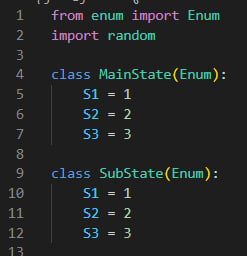
\includegraphics{1.jpg}
	\caption{
		این بخش مربوط به تعریف ورودی‌‌ها و انواع متغیرهای شمارشی (\texttt{Enum}) است. 
		دو \texttt{Enum} به نام‌های \texttt{MainState} و \texttt{SubState} تعریف شده‌اند که هر کدام سه حالت 
		\lr{(S1, S2, S3)}
		 دارند.
	}
	\label{fig:label1}
\end{figure}

\begin{figure}[h]
	\centering
	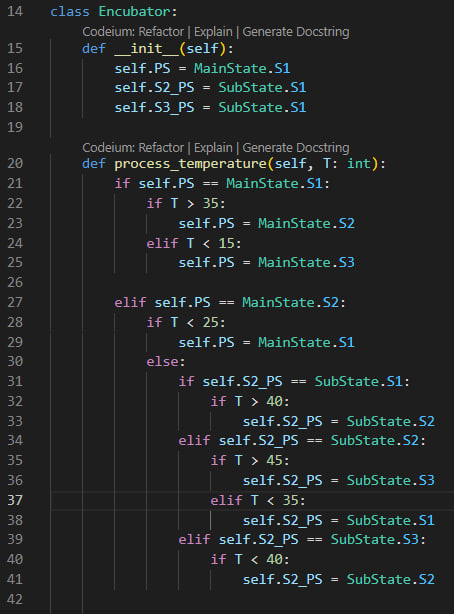
\includegraphics{2.jpg}
	\caption{اینجا یک کلاس به نام \texttt{Encubator} تعریف شده است که متدها و ویژگی‌های اولیه‌ی آن در این قسمت آورده شده. متد \texttt{process\_temperature} بر اساس دمای ورودی حالت‌های مختلف را مدیریت می‌کند و بر اساس دما، حالت‌های اصلی و زیر حالت‌ها را تغییر می‌دهد.}
	\label{fig:label2}
\end{figure}

\begin{figure}[h]
	\centering
	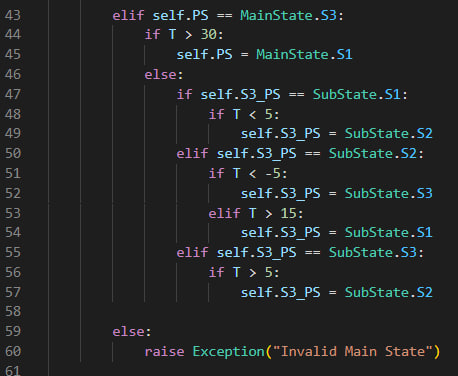
\includegraphics{3.jpg}
	\caption{این قسمت ادامه‌ی تابع \texttt{process\_temperature} است و به مدیریت حالت 
		\lr{S3}
	می‌پردازد. اگر دما یا حالتی خارج از حالت‌های تعریف شده باشد، یک خطا به کاربر نشان داده می‌شود.}
	\label{fig:label3}
\end{figure}

\begin{figure}[h]
	\centering
	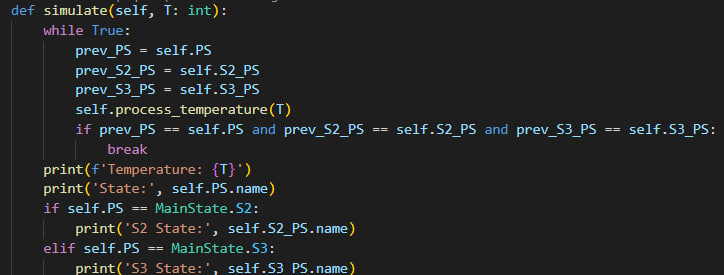
\includegraphics{4.jpg}
	\caption{متد \texttt{simulate} تعریف شده است که وظیفه‌ی آن شبیه‌سازی واکنش حالت‌ها به دما است. در این متد، تا زمانی که هیچ تغییری در حالت‌ها ایجاد نشود، پردازش دما ادامه می‌یابد. در نهایت، دما و حالت‌های فعلی نمایش داده می‌شوند.}
	\label{fig:label4}
\end{figure}

\begin{figure}[h]
	\centering
	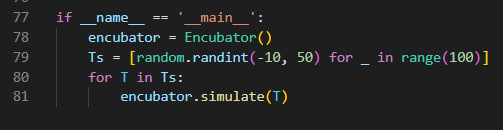
\includegraphics{5.jpg}
	\caption{این بخش کد اصلی برنامه است که یک نمونه از کلاس \texttt{Encubator} ایجاد می‌کند و سپس 100 دمای تصادفی می‌سازد و برای هر دما، شبیه‌سازی را اجرا می‌کند.}
	\label{fig:label5}
\end{figure}